\chapter{Ionización de átomos y moléculas: método de inversión depurada}
\label{chap:iondim}

%%%%%%%%%%%%%%%%%%%%%%%%%%%%%%%%%%%%%%%%%%%%%%%%%%%%%%%%%%%%%%%%%%%%%%%%
\section{Introducción}
%%%%%%%%%%%%%%%%%%%%%%%%%%%%%%%%%%%%%%%%%%%%%%%%%%%%%%%%%%%%%%%%%%%%%%%%

Los procesos inelásticos que se producen debido al impacto de diversos 
proyectiles se 
han estudiado de forma extensa en la teoría cuántica. A grandes rasgos, 
los métodos desarrollados para predecirlos se pueden clasificar en dos 
grupos: las aproximaciones perturbativas, entre las que se destacan las 
de Born~\cite{Bates:62,McDowell:61} y de onda 
distorsionada~\cite{Crothers:10,Rivarola:87}, y el grupo de métodos 
completamente cuánticos~\cite{Pindzola:07,Burke:11,Bray:17,
Zatsarinny:04,McCurdy:04}. 
Para calcular correctamente las probabilidades de transición en una 
colisión inelástica, es preciso representar adecuadamente los estados 
iniciales y finales del blanco. En general, la estructura de sistemas 
atómicos multielectrónicos se obtiene de resolver las ecuaciones de 
Schr\"odinger en el marco del modelo de partículas independientes en 
conjunción con la aproximación de campo central~\cite{Bransden:03,
Cowan:81}. 
\begin{comment}
Para calcular correctamente las probabilidades de transición en una 
colisión inelástica, es preciso representar adecuadamente los estados 
iniciales y finales del blanco. En general, la resolución de las 
ecuaciones de Schr\"odinger de sistemas multielectrónicos atómicos 
implementa el modelo de partículas independientes en conjunción con la 
aproximación de campo central~\cite{Bransden:03,Cowan:81}. 

La descripción de la estructura electrónica de sistemas moleculares 
constituye un desafío desde el punto de vista teórico debido a su 
geometría multicéntrica. Sin embargo, se han propuesto diversas 
aproximaciones para tal fin~\cite{Helgaker:00,Schaefer:04}. 

En el marco de la teoría cuántica, los procesos colisionales de átomos 
y moléculas simples debido al impacto de diversos proyectiles se ha 
estudiado de forma extensa. A grandes rasgos, los métodos desarrollados
para predecirlos se puden clasificar en dos grupos: las aproximaciones 
perturbativas, entre las que se destacan las de Born~\cite{Bates:62,
McDowell:61} y de onda distorcionada~\cite{Crothers:10,Rivarola:87}, y 
el grupo de métodos no perturbativos, con técnicas tales como los de 
acoplamiento cercano~\cite{Pindzola:07,Burke:11,Bray:17,Zatsarinny:04,
McCurdy:04}. 
\end{comment}

Los procesos colisionales simples se basan usualmente en la 
aproximación de electrón activo. En la ionización, el electrón activo 
está inicialmente ligado y luego de la colisión se encuentra libre. La 
descripción de los estados ligados es relativamente simple mientras que 
la representación de los continuos presenta cierta dificultad. Se han 
desarrollado diversas metodologías para el diseño de potenciales 
efectivos en blancos atómicos~\cite{Hibbert:82,Gombas:56,Green:69,
Klapisch:71,Phillips:59,Herman:63,Dalgarno:70,Bayliss:77,Cowan:76,
Lee:77} y moleculares~\cite{Menchero:10,Granados:16}. Es conveniente 
contar con un potencial efectivo local ya que permite obtener en forma 
consistente las funciones de onda de las partículas interactuantes. 
En este trabajo se estudia el método de inversión, que consiste en 
determinar potenciales centrales a partir de funciones de onda y/o 
densidades electrónicas. Este procedimiento se ha estudiado en la 
teoría del funcional de la densidad~(\acs{dft}, por sus siglas en 
inglés), en donde se emplean densidades del estado 
fundamental~\cite{Wu:03,Gaiduk:13,Ryabinkin:15,Schipper:97,deSilva:12,
Kananenka:13,Jacob:11}. El método 
de inversión fue sugerido por Hilton~\textit{et al.}, limitando su 
aplicaciones al cálculo de procesos de fotoionización~\cite{Hilton:77,
Suzer:77,Hilton:79,Hilton:80,Crljen:87}. A su vez, estos estudios se 
refieren a investigaciones previas en polarizabilidad 
atómica~\cite{Sternheimer:54,Dalgarno:59}. Sin embargo, estos trabajos 
se enfocan en los resultados de secciones eficaces y no presentan 
detalles acerca de la calidad de los potenciales y las funciones de onda 
resultantes. 

En este capítulo se estudia la estructura de átomos y moléculas pequeñas. 
La descripción de los blancos se obtiene a partir de potenciales que 
resultan de la implementación del \textbf{Método de Inversión 
Depurada}~(\acs{dim}). 
%El desarrollo teórico de esta técnica se presenta en la 
%Sección~\ref{sec:dimatomos}. El DIM consiste en la inversión de 
%ecuaciones de un electrón, cuyas soluciones se conocen. 
%Los potenciales resultantes se ajustan mediante expresiones 
%analíticas con las condiciones de borde apropiadas y se optimizan 
%variando los parámetros que los definen. El método de inversión depurada 
%es general y se puede aplicar a soluciones que se obtienen en el marco 
%de diversas aproximaciones. Con el fin de ilustrar su implementación, 
%las soluciones que se utilizan en este trabajo están dadas por la 
%teoría de Hartree--Fock~(\acs{hf}). La utilización de orbitales de HF en 
%el DIM se presenta en la Sección~\ref{subsec:invHF}. Si bien el 
%procedimiento de inversión es directo, los potenciales resultantes 
%presentan polos y divergencias. El origen de estos defectos se discuten 
%al final de este Capítulo, en la Sección~\ref{sec:discusionHF}. Como 
%corolario del DIM con orbitales HF, y asumiendo la 
%validez de la separación de los términos de intercambio y correlación, 
%en la Sección~\ref{sec:corolarios} se presentan potenciales de 
%intercambio ``exactos''. A partir de los potenciales DIM también se 
%pueden calcular las energías totales y de intercambio de forma directa. 
El objetivo principal de este capítulo es ilustrar el uso efectivo de 
potenciales DIM en la teoría de colisiones atómicas. Para este fin 
se realizan ciertas simplificaciones: los cálculos están restringidos a 
los Hamiltonianos que describen el proyectil, el blanco y el electrón 
activo, y los elementos de la matriz de transición se consideran en 
primer orden perturbativo. 
Así, el marco teórico de los procesos colisionales estará dado por la 
primera aproximación de Born (FBA), que reproduce razonablemente las 
secciones eficaces experimentales de diversos procesos en el rango 
intermedio--alto de energías incidentes del proyectil. 

%Los resultados de la implementación del método de inversión depurada 
%para describir la estructura de blancos atómicos y moleculares se 
%presentan en la Sección~\ref{subsec:dimtarget}. La uso efectivo del DIM 
%se evalúa a partir de la descripción de la estructura electrónica del 
%blanco y la predección del proceso colisional al que son sometidos. Las 
%valores teóricos resultantes de la combinación de los 
%potenciales DIM y la FBA para describir la ionización simple de átomos y 
%moléculas por impacto de protones y fotones se muestra en la 
%Sección~\ref{subsec:procol}. Las conclusiones de este trabajo se 
%encuentran en la Sección~\ref{sec:conclu-dim}. En la presentación de 
%esta Tesis, se examinan resultados de cuatro blancos: helio, nitrógeno, 
%neón y metano. Sin embargo, hemos presentado una gran cantidad de 
%potenciales DIM en diversas publicaciones en los últimos 
%años~\cite{Mendez:16,Mendez:19dim,Mendez:18}. 
%Además, actualmente continuamos trabajando en una base de 
%datos de estructura de átomos y potenciales que cubre todos los 
%elementos no relativistas de la tabla periódica, que será de libre 
%acceso. 

%%%%%%%%%%%%%%%%%%%%%%%%%%%%%%%%%%%%%%%%%%%%%%%%%%%%%%%%%%%%%%%%%%%%%%%%
\section{Método de inversión depurada (DIM)}
%%%%%%%%%%%%%%%%%%%%%%%%%%%%%%%%%%%%%%%%%%%%%%%%%%%%%%%%%%%%%%%%%%%%%%%%
\label{sec:dimatomos}

La ecuación de Schr\"odinger de un sistema de $N$ electrones y carga $Z$ 
en la aproximación de campo central está dada por
\begin{equation}
 \left[ -\frac{1}{2}\frac{d^2}{dr^2} + \frac{l(l+1)}{2r^2} +
 V(r) \right] u_{nl}(r) = \varepsilon_{nl} \, u_{nl}(r)\,,
\label{eq:eqSchroRadial}
\end{equation}
donde $V(r)$ es el potencial que gobierna la dinámica, $u_{nl}$ es la 
función radial reducida y $\varepsilon_{nl}$ la energía del orbital 
$nl$. 
El método de inversión depurada consiste en resolver el problema inverso
de la Ec.~(\ref{eq:eqSchroRadial}): suponiendo que las soluciones 
$u_{nl}$ y $\varepsilon_{nl}$ se conocen, es posible definir un 
\textit{potencial invertido} que las generan
\begin{equation}
V_{nl}(r) = 
\frac{1}{2}\frac{1}{u_{nl}(r)} \frac{d^2\,u_{nl}(r)}{dr^{2}} - 
\frac{l(l+1)}{2r^{2}}+\varepsilon_{nl} \,.
\label{eq:Vinv}
\end{equation}

Asumiendo que el potencial invertido tienen una forma Coulombiana, 
es conveniente definir una \textit{carga invertida} tal que
\begin{equation}
Z_{nl}(r) \equiv -r \, V_{nl}(r) \,.
\label{eq:Zinv}
\end{equation}
El comportamiento general del potencial y de su correspondiente carga 
efectiva se ilustran en la Fig.~\ref{fig:potycharge}; la carga deberá 
ser suave y cumplir con condiciones de borde definidos por la naturaleza 
del blanco a describir: 
en el origen la carga debe ser igual a la carga nuclear del átomo y 
asintóticamente, debido al apantallamiento electrónico, ésta debe ser
igual a uno. Esto es,
\begin{equation}
Z_{nl}(r) \, \rightarrow 
\bigg\{ 
\begin{array}{ll}
Z  \ \  & \ \ \text{:\ \ }r  \rightarrow 0 \,, \\ 
1           & \ \ \text{:\ \ }r  \rightarrow \infty \,.
\end{array}
\label{eq:Zasympt}
\end{equation} 
En el DIM, la carga invertida se ajusta con una expresión analítica que 
cumple con estas condiciones de borde.

\begin{figure}[t]
\centering
\includegraphics[width=0.93\textwidth]{dim/pot-charge.eps}
\caption[Características físicas del potencial y carga efectiva.]
{Ilustración de las características físicas esperadas del (a) potencial 
y (b) carga efectiva para el átomo de carga nuclear $Z$.}
\label{fig:potycharge}
\end{figure}

Debido a la presencia de la función de onda en el denominador de la 
Ec.~(\ref{eq:Vinv}), es posible que las cargas invertidas presenten 
defectos numéricos. De ser así, se restringe la región de ajuste 
descartando comportamientos inconsistentes con la naturaleza del blanco,
tales como polos o divergencias. En átomos, la carga DIM está dada por
\begin{equation}
Z_{nl}^{\mathrm{DIM}}(r)= \sum_{j=1}^{n} z_j e^{-\alpha_j r}+1 \,,
\label{eq:atomzDIM}
\end{equation}
donde $\Sigma_j z_j=Z-1$. Los parámetros $\left\{z_j,\alpha_j\right\}$ 
definen un potencial de prueba que se optimiza hasta reproducir las 
soluciones iniciales $u_{nl}$ y $\varepsilon_{nl}$ de manera precisa. 

La mayoría de los métodos de funcional de la densidad están basados en 
un principio variacional que minimiza la energía. Sin 
descartar su importancia, la energía es solo uno de los observables que 
caracteriza un estado cuántico. Más aún, a partir de diferentes 
funciones de prueba (de formas variadas) e implementando un método 
variacional, es posible reproducir la misma energía final. Por ejemplo, 
Bartschat \textit{et al.}~\cite{Albright:93,Bartschat:96} muestra que 
dos potenciales diferentes (uno conteniendo intercambio electrónico y 
otro despreciándolo) conducen a energías similares y precisas de la 
serie de Rydberg en varios sistemas de cuasi-un electrón. Sin embargo, 
estos potenciales conducen a grandes discrepancias cuando se implementan 
en cálculos de dispersión \cite{BartschatBray:96}. Por lo tanto, además 
de los valores de energía, se incluyen en la optimización DIM valores 
medios de $\langle r^k \rangle$, tal que $k=-1,1$. La inclusión de estos 
observables permite caracterizar la precisión del orbital DIM cerca 
($k=-1$) y lejos ($k=1$) del origen. Así, la función de costo $J$ que se 
define para la optimización de los potenciales DIM está dada por los 
errores relativos de cada una de estas cantidades
\begin{equation}
J=\sum_{i=1}^3 \frac{X_i-\widebar{X}_i}{X_i}\,,
\label{eq:fncosto-dim}
\end{equation}
donde la suma se hace sobre 
$X=\left[\varepsilon,\langle r \rangle,\langle 1/r \rangle\right]$, 
siendo $X$ los valores conocidos y $\widebar{X}$ los resultados que se 
obtienen de resolver la Ec.~(\ref{eq:eqSchroRadial}) con el potencial 
paramétrico. 

La variación del conjunto de parámetros $\left\{z_j,\alpha_j\right\}$ no 
es sistematizable mediante métodos convencionales debido a tres 
características del problema. En primer lugar, el hiper-espacio de 
parámetros que se define consta de entre 3 y 7 dimensiones. De manera 
que la implementación de muchas técnicas de optimización, tales como 
búsqueda de grilla, resultan numéricamente impracticables. Además,
la función de costo no está dada por una función analítica, por lo que 
las técnicas basadas en el gradiente de la función también se descartan. 
Finalmente, la hiper-superficie definida por el costo no es convexa; de 
manera que la aplicación de métodos convencionables, que no dependen de 
la derivada, generalmente sólo encuentran mínimos locales. Por estos
motivos, el ajuste sólo puede hacerse en forma manual, lo que requiere 
requiere habilidad, pericia y experiencia. Actualmente, la autora y 
colaboradores se encuentran trabajando en incorporar métodos de 
optimización usados en el campo del aprendizaje automatizado en el 
DIM~\cite{DiFilippo:19}.

%%%%%%%%%%%%%%%%%%%%%%%%%%%%%%%%%%%%%%%%%%%%%%%%%%%%%%%%%%%%%%%%%%%%%%%%
\subsection{DIM y soluciones Hartree--Fock}
%%%%%%%%%%%%%%%%%%%%%%%%%%%%%%%%%%%%%%%%%%%%%%%%%%%%%%%%%%%%%%%%%%%%%%%%
\label{subsec:invHF}

El método de inversión depurada es general y se puede implementar con 
soluciones que se obtienen en el marco de diversas aproximaciones. Con 
el fin de ilustrar su aplicación, en esta presentación se usan 
soluciones obtenidas mediante la teoría de Hartree--Fock. La utilización 
del método HF presenta una gran ventaja: la teoría se conoce en detalle 
y se obtienen soluciones 
con gran precisión. De esta forma, se puede hacer una comparación 
estricta con el DIM y sus resultados, verificando la calidad de los 
potenciales que proporciona el método.

\begin{figure}[t]
\centering
\includegraphics[width=0.88\textwidth]{dim/dim_2sK.eps} 
\caption[Orbital radial y carga efectiva correspondiente.]
{(a) Orbital radial $u_{2s}^{\mathrm{HF}}$ del estado fundamental de K.
(b) Cargas invertida $Z_{2s}^{\mathrm{HF}}$ (línea discontinua) 
y depurada $Z_{2s}^{\mathrm{DIM}}$ (línea sólida).}
\label{fig:2sK}
\end{figure}

A pesar de que el procedimiento de inversión dado por la 
Ec.~(\ref{eq:Vinv}) es directo, su implementación a partir de las 
soluciones HF no produce, en general, cargas invertidas suaves. Por 
ejemplo, en la Fig.~\ref{fig:2sK} se muestra (a)~el orbital 
$u_{2s}^{\mathrm{HF}}$ del átomo de potasio en su estado fundamental y 
(b) su correspondiente carga invertida $Z_{2s}^{\mathrm{HF}}$ (línea 
discontinua). También se muestra la carga $Z_{2s}^{\mathrm{DIM}}$ (línea 
sólida), que se obtiene luego de ajustar la carga invertida mediante la 
Ec.~(\ref{eq:atomzDIM}). El orbital $2s$ tiene dos nodos: un nodo 
genuino en $r\approx 0.111$~a.u. y un nodo espurio en 
\mbox{$r\approx 5.79$~a.u.}. Se usa el término genuino para denotar los 
nodos que cumplen la relación del número cuántico radial $n_r=n-l-1$. 
Por otro lado, los nodos espurios no han suscitado demasiada atención 
porque aparecen a grandes distancias, en regiones donde la amplitud del 
orbital es muy pequeña. Ambos nodos son traducidos a la carga invertida 
como polos. La inversión directa produce otro problema numérico que la 
torna inutilizable; $Z_{2s}^{\mathrm{HF}}$ presenta una 
divergencia pronunciada para grandes distancias radiales (en la figura, 
por ejemplo, para $r\geq 1$~a.u.). 

\begin{figure}[t]
\centering
\begin{tikzpicture}[remember picture]
%  \tikzset{shift={(current page.center)}}
\node[process,fill=green!15] (inv) 
          {Inversión directa};
\node[process] (region) at (inv) [xshift=0cm,yshift=-1.5cm] 
          {Definición de región de ajuste};
\node[process] (eqnorm) at (region) [xshift=0cm,yshift=-1.5cm] 
          {Definición de semillas};
\node[process,text width=4.8cm] (diag) 
          at (eqnorm) [xshift=0cm,yshift=-2cm] 
          {Diagonalización y \\cálculo de
          valores medios};
\node[process] (costo) at (diag) [xshift=-2.5cm,yshift=-2.3cm] 
          {Cálculo de costo};
\node[process] (var) at (diag) [xshift=2.5cm,yshift=-2.3cm] 
          {Variación de parámetros};
\node[decision] (converge) at (costo) [xshift=-4cm,yshift=0cm] 
          {¿Convergió?};
\node[process,fill=blue!20] (dim) at (diag) [xshift=0cm,yshift=-5.2cm] 
          {Potencial DIM};
\draw[arrow] (inv) -- (region);
\draw[arrow] (region) -- (eqnorm);
\draw[arrow] (eqnorm) -- (diag);
\draw[arrow,bend right=33] (diag.west) 
                        to ([xshift=-0.75cm,yshift=0cm]{costo.north});
\draw[arrow,bend right=53] ([xshift=-0.3cm,yshift=0cm]{costo.south}) 
                        to ([xshift=0.3cm,yshift=0cm]{var.south});
\draw[arrow,bend right=33] ([xshift=0.75cm,yshift=0cm]{var.north}) 
                        to (diag.east);
\draw[arrow,dashed] (costo) -- (converge);
\draw[arrow,dashed] (converge) |- (region.west) node [near start,left] 
                    {No};
\draw[arrow,dashed] (converge) |- (dim.west) node [near start,right] 
                    {Sí};
\end{tikzpicture}
\caption{Procedimiento de optimización del potencial DIM.}
\label{fig:procDIM}
\end{figure}

La justificación numérica a la presencia de los polos es simple: surgen 
por la presencia del nodo del orbital radial $2s$ en el denominador de 
la Ec.~(\ref{eq:Vinv}). Por otro lado, la divergencia asintótica en la 
carga se estudia más adelante, en la Sección~\ref{sec:discusionHF}. 
En general, las cargas resultantes de la inversión de orbitales HF 
tienen asociadas alguno de estos defectos. 

El procedimiento general para la obtención de los potenciales DIM a 
partir de orbitales HF se esquematiza en la Fig.~\ref{fig:procDIM}. Para 
el orbital $nl$ de un blanco dado, se implementa la Ec.~(\ref{eq:Vinv}). 
Primero, se define una región de ajuste sobre la carga invertida 
resultante. La clave de una optimización exitosa está dada por la 
correcta definición de esta región: tiene que ser lo más extensa 
posible, descartando por completo cualquier defecto numérico. La segunda 
parte de la optimización consiste en definir una semilla inicial para 
los parámetros $\left\{z_j,\alpha_j\right\}$. Se sabe que en un proceso 
de optimización, la elección de estos valores es fundamental. En este 
trabajo, las semillas se obtienen mediante la resolución de la ecuación 
normal definida por el problema (ver detalles en 
Apéndice~\ref{app:ecnormal}). Los valores resultantes determinan un 
potencial de prueba con el que se resuelve la 
Ec.~(\ref{eq:eqSchroRadial}). A partir de las soluciones de la 
diagonalización se calculan los valores medios que definen la función de 
costo~(\ref{eq:fncosto-dim}), que se minimiza variando los parámetros 
del problema en forma iterativa. Cuando las soluciones del potencial de 
prueba convergen a los valores de HF de forma correcta, estos parámetros 
se definen como los parámetros del potencial DIM. En el caso que las 
soluciones no convergan a los valores correctos, se reinicia el 
procedimiento redefiniendo la región de ajuste de la carga invertida.

%%%%%%%%%%%%%%%%%%%%%%%%%%%%%%%%%%%%%%%%%%%%%%%%%%%%%%%%%%%%%%%%%%%%%%%%
\subsection{Corolarios de DIM-HF}
%%%%%%%%%%%%%%%%%%%%%%%%%%%%%%%%%%%%%%%%%%%%%%%%%%%%%%%%%%%%%%%%%%%%%%%%
\label{sec:corolarios}

%=======================================================================
\subsubsection*{Energía total}
%=======================================================================

A partir de la definición de energía total del sistema dada por la 
teoría de Hartree--Fock, es posible derivar una expresión 
correspondiente en el marco del método de inversión depurada. Así, la 
energía total DIM se expresa en términos del potencial DIM y sus 
soluciones como
\begin{equation}
E^{\mathrm{DIM}} = \sum\limits_{nl} 
\left[ 
\varepsilon_{nl}^{\mathrm{DIM}} - 
\frac{1}{2}\int  \rho_{nl}^{\mathrm{DIM}}(r)
\left( V_{nl}^{\mathrm{DIM}}(r) + \frac{Z_{N}}{r}\right) dr \,
\right] \, ,
\label{eq:Etotal}
\end{equation}
donde la densidad es 
$\rho_{nl}^{\mathrm{DIM}}(r)=|u_{nl}^{\mathrm{DIM}}(r)|^2$. 

Como se ha visto, los potenciales orbitales $nl$ de un átomo en el DIM 
se optimizan de forma independiente. El cálculo de la energía total del 
estado fundamental del sistema dado por la Ec.~(\ref{eq:Etotal}) permite 
evaluar la optimización de estos potenciales en forma global.

%=======================================================================
\subsubsection*{Potenciales de intercambio}
%=======================================================================

En la teoría de Hartree--Fock, es posible determinar el potencial de 
intercambio orbital de un blanco aplicando el operador de Fock. Sin 
embargo, el potencial resultante no es local ya que depende del resto de 
los orbitales. La primera aproximación local fue propuesta por 
Slater~\cite{Slater:51}, en la cual se obtiene un potencial de 
intercambio promediado a partir de la densidad de carga de intercambio 
promedio. Otra aproximación, propuesta por Sharp y 
Horton~\cite{Sharp:53}, consiste en aproximar el operador de intercambio 
utilizando un potencial local, y minimizando la energía mediante un 
método variacional donde se minimiza 
la energía. Desde entonces, se han desarollado diversos métodos más 
elaborados que permiten determinar potenciales de 
intercambio~\cite{Krieger:92,Gorling:92,Yang:02,Staroverov:06,
Ryabinkin:13}. Sin embargo, estos potenciales son difíciles de expresar 
mediante fórmulas analíticas simples y no se pueden implementar en 
problemas colisionales como los que se tratan en este trabajo.

Debido a que la teoría de Hartree--Fock incluye el término de 
intercambio electrónico de manera exacta, el método de inversión 
depurada permite definir potenciales ``exactos'' 
$V_{nl}^{\mathrm{x}}(r)$ para cada orbital $nl$. Suponiendo que el 
potencial DIM se puede expresar como
\begin{equation}
V_{nl}^{\mathrm{DIM}}(r) = -\frac{Z}{r} + V^{\mathrm{H}}(r) 
+ V_{nl}^{\mathrm{x}}(r) \, , 
\label{eq:VDIM}
\end{equation}
donde $V^{\mathrm{H}}$ es el potencial directo local debido a la 
repulsión electrostática electrónica en el esquema de HF y 
$V_{nl}^{\mathrm{x}}$ es el potencial de intercambio orbital. Entonces,
\begin{equation}
V_{nl}^{\mathrm{x}}(r)=V_{nl}^{\mathrm{DIM}}(r)+\frac{Z}{r}
-\int{ \frac{\rho^{\mathrm{HF}}(r^{\prime})  }
{\left| \mathbf{r} - \mathbf{r^{\prime}} \right|}} \, 
d \mathbf{r^{\prime}} \, ,
\label{eq:exchange-potential}
\end{equation}
donde $\rho^{\mathrm{HF}}$ es la densidad electrónica total que se
calcula a partir de los orbitales HF.

%=======================================================================
\subsubsection*{Energías de intercambio}
%=======================================================================

A partir de los potenciales de intercambio DIM, se puede definir la 
energía de intercambio total DIM $E^{\mathrm{x}}$ como
\begin{equation}
E^{\mathrm{x}} = \sum_{nl}\varepsilon_{nl}^{\mathrm{x}} = 
\sum_{nl}\left[\frac{1}{2}\int{\rho^{\mathrm{HF}}_{nl}(r) \, \, 
V_{nl}^{\mathrm{x}}}(r) \, dr \, \right]\,,
\label{eq:exchange-energy}
\end{equation}
donde $\varepsilon_{nl}^{\mathrm{x}}$ son las energías de intercambio 
correspondiente a cada orbital $nl$. La expresión de la energía de 
intercambio total DIM permite comparar la calidad de los 
potenciales~(\ref{eq:exchange-potential}) con valores de referencia. 
En definitiva, esta relación representa una cantidad adicional con la 
que se puede evaluar cuantitativamente al método.

%%%%%%%%%%%%%%%%%%%%%%%%%%%%%%%%%%%%%%%%%%%%%%%%%%%%%%%%%%%%%%%%%%%%%%%%
\section{DIM en moléculas}
%%%%%%%%%%%%%%%%%%%%%%%%%%%%%%%%%%%%%%%%%%%%%%%%%%%%%%%%%%%%%%%%%%%%%%%%
\label{sec:dimmoleculas}

El método de inversión depurada se puede extender para obtener 
potenciales efectivos para moléculas simples. Para ello, primero se 
define el método mediante el cual se obtienen los orbitales moleculares.
Luego, se plantea el esquema de inversión de las soluciones y la 
extensión al método de depuración con el que se obtienen los potenciales 
moleculares. 

%%%%%%%%%%%%%%%%%%%%%%%%%%%%%%%%%%%%%%%%%%%%%%%%%%%%%%%%%%%%%%%%%%%%%%%%
\subsection{Descripción de moléculas}
%%%%%%%%%%%%%%%%%%%%%%%%%%%%%%%%%%%%%%%%%%%%%%%%%%%%%%%%%%%%%%%%%%%%%%%%
\label{sec:moleculas}

La descripción de la estructura electrónica de sistemas moleculares 
constituye un desafío desde el punto de vista teórico debido a su 
geometría multicéntrica~\cite{Helgaker:00,Schaefer:04}. 
En el marco de la aproximación de Born--Oppenheimer, el Hamiltoniano 
molecular no--relativista en el que sólo se consideran fuerzas 
Coulombianas puede escribirse como
\begin{equation}
H=-\sum_{i=1}^N \frac{1}{2} \nabla^2_{\mathbf{r}_i} 
  +\sum_{i<j=1}^N \frac{1}{\left|\mathbf{r}_i-\mathbf{r}_j\right|} 
  -\sum_{i=1}^N \sum_{\alpha=1}^n \frac{Z_{\alpha}}{
    \left|\mathbf{r}_i-\mathbf{r}_{\alpha}\right|} 
%  +\sum_{\alpha<\beta=1}^n \frac{z_{\alpha}z_{\beta}}{
%         \left|\mathbf{r}_{\alpha}-\mathbf{r}_{\beta}\right|}\,,
\label{eq:BOhamiltonian}
\end{equation}
donde los índices $i,j$ van sobre todos los electrones y $\alpha$ 
sobre todos los núcleos. 
Teniendo en cuenta las mismas razones esgrimidas en el caso atómico, la 
ecuación de Schr\"odinger correspondiente, $H\Psi=E\Psi$, se resuelve a 
partir del método de Hartree--Fock, y el sistema de ecuaciones 
resultantes implementa bases finitas para la representación de los 
orbitales moleculares. Estos orbitales se expresan como una combinación 
lineal de orbitales atómicos, 
tal que
\begin{equation}
\Psi_i(\mathbf{r})=\sum_j c_{ji} \phi_j(\mathbf{r})\,.
\end{equation}
A su vez, los orbitales atómicos $\phi(\mathbf{r})$ se construyen a 
partir de conjuntos de base, por ejemplo, de orbitales tipo Gaussianos. 
La construcción de los orbitales moleculares a partir de estas funciones 
es conveniente ya que el producto de dos Gaussianas centradas en dos 
átomos diferentes resulta en una suma finita de Gaussianas centradas en 
un punto a lo largo del eje que las conecta. De esta manera, las 
integrales de múltiples centros se pueden reducir significativamente, lo 
que proporciona una gran ventaja computacional.

%%%%%%%%%%%%%%%%%%%%%%%%%%%%%%%%%%%%%%%%%%%%%%%%%%%%%%%%%%%%%%%%%%%%%%%%
\subsection{Inversión con bases Gaussianas}
%%%%%%%%%%%%%%%%%%%%%%%%%%%%%%%%%%%%%%%%%%%%%%%%%%%%%%%%%%%%%%%%%%%%%%%%
\label{sec:invmol}

En general, los orbitales moleculares se expanden alrededor de los 
núcleos atómicos que componen la molécula. A partir de la utilización
de orbitales de tipo Gaussianos esféricos, los orbitales moleculares se 
expanden en un único centro y la expresión del potencial molecular 
invertido es análoga a la Ec.~(\ref{eq:Vinv}). 

La representación de los orbitales moleculares por conjuntos de base de 
orbitales tipo Gaussianos introduce nuevas dificultades numéricas en el 
procedimiento de inversión. Además de las divergencias asintóticas y los 
polos, los potenciales invertidos moleculares presentan grandes 
oscilaciones~\cite{Schipper:97,Jacob:11,Gaiduk:13}. Estas oscilaciones 
prominentes aparecen por la presencia de ondulaciones en los orbitales 
moleculares, que a su vez surgen debido al número finito de elementos en 
la base. La segunda derivada de los orbitales, necesaria para evaluar la 
fórmula inversa, amplifica estos rasgos. En algunos casos, las 
oscilaciones son enormes; por ejemplo, cerca de átomos electronegativos 
como el cloro. La aparición de estas oscilaciones en los potenciales 
invertidos requiere el desarrollo de nuevas técnicas de depuración.

%%%%%%%%%%%%%%%%%%%%%%%%%%%%%%%%%%%%%%%%%%%%%%%%%%%%%%%%%%%%%%%%%%%%%%%%
\subsection{Depuración y perfiles de oscilación}
%%%%%%%%%%%%%%%%%%%%%%%%%%%%%%%%%%%%%%%%%%%%%%%%%%%%%%%%%%%%%%%%%%%%%%%%
\label{sec:invmol}

Los patrones de oscilación en los potenciales invertidos moleculares 
varían según el conjunto de base utilizado para representar las 
soluciones. Dado que los orbitales moleculares se expresan como 
combinación lineal de orbitales atómicos, se definen perfiles de 
oscilación por átomo, por base y por orbital. Para el átomo $\alpha$ que 
se describe implementando un conjunto de base (BS), el perfil de 
oscilación del orbital $nl$ está dado por
\begin{equation}
 p_{nl}^{\mbox{\scriptsize BS}} = Z_{nl}^{\mbox{\scriptsize BS}}-
 Z_{nl} \,,
 \label{eq:oscillation-prof}
\end{equation}
donde $Z_{nl}^{\mbox{\scriptsize BS}}$ es la carga invertida del orbital
$nl$ del átomo $\alpha$ cuando se usa el conjunto de bases ``BS'' y 
$Z_{nl}$ es la carga invertida correspondiente cuando los orbitales se 
obtienen mediante algún método de referencia en el cual desaparezcan 
(o en el cual se disminuyan notoriamente) estas oscilaciones. La 
implementación de la Ec.~(\ref{eq:oscillation-prof}) requiere que las 
soluciones usadas en la 
inversión estén dadas por el mismo esquema de aproximación (por ejemplo, 
la teoría de Hartree--Fock). De esta manera, nos aseguramos que las 
oscilaciones provienen exclusivamente del carácter limitado de la base
escogida.

Una vez que los $nl$ perfiles de oscilación atómicos de la base se 
definen, éstos se pueden sustraer de manera directa de los potenciales 
moleculares. Por ejemplo, en un hidruro XH$_n$, es necesario definir los 
perfiles de oscilación del átomo X y del hidrógeno. Luego, se implementa 
el procedimiento de depuración descripto para átomos. De acuerdo a la 
estructura de las moléculas consideradas, se definen expresiones 
analíticas particulares para diferentes grupos de compuestos. Por 
ejemplo, la ecuación parámetrica para las cargas moleculares DIM de 
hidruros se define como
\begin{eqnarray}
 Z(r) = \sum_j z_j e^{-\alpha_j r} 
 + z_{\mbox{\scriptsize H}} e^{-(\ln r - \ln \beta)^2/(2\gamma)} 
 + 1\,.
 \label{eq:molzDIM}
\end{eqnarray}
En contraste con la aproximación propuesta para los átomos, el segundo 
término en la expresión~(\ref{eq:molzDIM}) se incluye para tener en 
cuenta el efecto de carga producido por los hidrógenos. Este nuevo 
término permite ajustar convenientemente tanto la ubicación como el 
ancho de los potenciales hidrogénicos apantallados, sin afectar el valor 
correcto de la carga en el origen.

\begin{figure}[t]
\centering
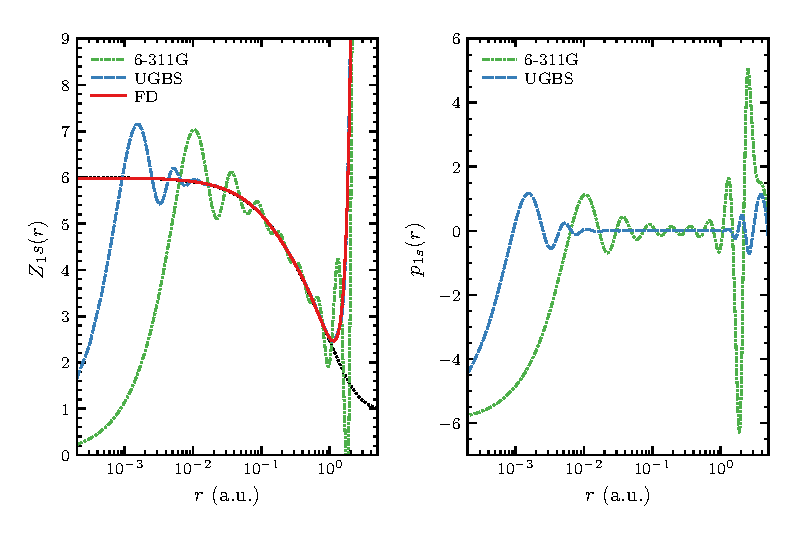
\includegraphics[width=0.9\textwidth]{dim/carbon_prof.eps}
\caption[Inversión de orbitales descriptos con conjuntos de base 
finitos.]
{(a) Cargas efectivas invertidas del orbital $1s$ del átomo de carbón.
(b)~Perfiles de oscilación de los conjuntos de base.}
\label{fig:1sCarbon}
\end{figure}

Para ilustrar este procedimiento, se considera el orbital $1s$ del átomo 
de carbono. Primero, se resuelven las ecuaciones de Hartree--Fock usando 
el conjunto de bases \mbox{6-311G} con el código 
\textsc{gamess}~\cite{Schmidt:93,Gordon:05}. Luego, aplicando la 
Ec.~(\ref{eq:Vinv}), se obtiene la carga invertida correspondiente. La 
carga resultante $Z_{1s}^{\mbox{\scriptsize 6-311G}}$ se muestra en la 
Fig.~\ref{fig:1sCarbon}(a) con una línea raya-punto verde. La carga 
tiene oscilaciones en toda su extensión radial, divergiendo para valores 
grandes de $r$. Se realiza el mismo cálculo con el conjunto de base 
universal Gaussiano (\acs{ugbs}), que tiene un número significativamente 
mayor de funciones primitivas. La carga invertida correspondiente 
$Z_{1s}^{\mbox{\scriptsize UGBS}}$ se presenta en la figura con una 
línea discontinua celeste. A pesar que la carga aún diverge cerca de 
$r\approx1\,$a.u., las oscilaciones en la región media desaparecen. 
Finalmente, se resuelven las ecuaciones diferenciales de Hartree--Fock 
para el átomo de carbono usando el método de diferencias finitas 
(\acs{fd}) con el código \textsc{hf} de C. Froese 
Fischer~\cite{FroeseFischer:97}. La carga invertida 
$Z_{1s}^{\mbox{\scriptsize FD}}$ correspondiente se exhibe con una línea 
sólida roja en la Fig.~\ref{fig:1sCarbon}(a). Como es de esperar, esta 
carga invertida no presenta oscilaciones, ya que no se utilizó una base 
para construir los orbitales. Sin embargo, la carga diverge para 
$r>1\,$a.u. debido a las características de la teoría de Hartree--Fock 
que se detallan en la Sección~\ref{sec:discusionHF}. Los perfiles de 
oscilación correspondiente al orbital $1s$ debido a los conjuntos de 
base \mbox{6-311G} y UGBS se obtienen a partir de la 
Ec.~(\ref{eq:oscillation-prof}) y se muestran en la 
Fig.~\ref{fig:1sCarbon}(b). Los perfiles de oscilación para un conjunto 
de base atómico son únicos. Una vez que se determinan, se pueden 
sustraen de los potenciales moleculares invertidos de manera directa. 
Luego, se implementa la Ec.~(\ref{eq:molzDIM}) y los parámetros 
se optimizan siguiendo la metodología presentada en la 
Sección~\ref{sec:dimatomos}.

%%%%%%%%%%%%%%%%%%%%%%%%%%%%%%%%%%%%%%%%%%%%%%%%%%%%%%%%%%%%%%%%%%%%%%%%
\section{Resultados}
%%%%%%%%%%%%%%%%%%%%%%%%%%%%%%%%%%%%%%%%%%%%%%%%%%%%%%%%%%%%%%%%%%%%%%%%
\label{sec:dimresultados}

A continuación se presentan los resultados obtenidos mediante la 
implementación del método de inversión depurada para describir blancos
atómicos y moleculares. El DIM se combina con la primera aproximación de 
Born para describir procesos inelásticos en blancos multielectrónicos. 
%Las secciones eficaces de ionización 
%predichas por el modelo se examinan mediante comparación con los datos 
%experimentales disponibles. 
A lo largo de este trabajo de investigación se han estudiado diversos 
blancos mediante el método DIM, publicados en las Refs.~\cite{Mendez:16,
Mendez:19dim,Mendez:18}. De estos resultados, se han seleccionado cuatro 
blancos para describir en detalle en esta Tesis: helio, nitrógeno, neón 
y metano.

%%%%%%%%%%%%%%%%%%%%%%%%%%%%%%%%%%%%%%%%%%%%%%%%%%%%%%%%%%%%%%%%%%%%%%%%
\subsection{Estructura electrónica de blancos}
%%%%%%%%%%%%%%%%%%%%%%%%%%%%%%%%%%%%%%%%%%%%%%%%%%%%%%%%%%%%%%%%%%%%%%%%
\label{subsec:dimtarget}

Las soluciones $u_{nl}^{\mathrm{HF}}$ y $\varepsilon^{\mathrm{HF}}$ de 
Hartree--Fock, que se implementan en la Ec.~(\ref{eq:Vinv}), se calculan 
usando indistintamente los códigos \textsc{hf} de C. Froese 
Fischer~\cite{FroeseFischer:97}, y \textsc{nrhf} de W. 
Johnson~\cite{Johnson:07}. Si bien ambos códigos resuelven la estructura
de blancos no relativistas utilizando diferencias finitas, los 
algoritmos, métodos y grillas numéricas utilizadas son diferentes. 

%=======================================================================
\subsubsection{Helio}
%=======================================================================

En primer lugar, se muestran los resultados obtenidos al implementar
el método de inversión depurada en el átomo de helio en su estado
fundamental. La inversión del orbital $1s$ no presenta ningún defecto
de los descriptos en la Sección~\ref{subsec:invHF}. Además, la 
simplicidad del blanco nos permite ajustar la carga invertida con un 
número reducido de parámetros. La carga invertida $Z_{1s}^{\mathrm{HF}}$ 
y la carga invertida depurada $Z_{1s}^{\mathrm{DIM}}$ se muestran en la 
Fig.~\ref{fig:Hepots}(a) con línea discontinua y sólida, 
respectivamente. La carga DIM descripta por la Ec.~(\ref{eq:atomzDIM}), 
se puede optimizar con sólo tres parámetros, los cuales se dan en la 
Tabla~\ref{tab:params-atoms}. 

\begin{figure}[t]
\centering
\includegraphics[width=0.9\textwidth]{figures/dim/Hepots.eps}
\caption[Cargas efectivas y potencial de intercambio DIM de He.]
{(a) Cargas efectivas $1s$ del He ($^1$S) obtenidas mediante inversión 
directa (línea discontinua) e inversión depurada (línea sólida). 
(b) Potencial de intercambio DIM (línea sólida) y OPM (línea punteada).}
\label{fig:Hepots}
\end{figure}

Para verificar la calidad de la estructura atómica dada por el potencial 
DIM, en la Tabla~\ref{tab:results-atoms} se presenta una comparación 
de los valores de energías total y orbital, y los radios medios 
obtenidos utilizando el método de inversión depurada (fila superior) con 
sus correspondientes valores originales de Hartree--Fock (fila 
inferior). El potencial DIM reproduce el valor de energía total, dada 
por la Ec.~(\ref{eq:Etotal}), en un $0.003\%$. La energía orbital $1s$ 
coincide con la energía de HF en 6 cifras significativas. Los valores 
medios de $u_{1s}^{\mathrm{DIM}}$ también muestran una excelente 
concordancia, tanto para la región cercana al origen, 
$\langle 1/r\rangle$, como en la región lejana, $\langle r\rangle$.

El potencial de intercambio orbital DIM del átomo de helio, definido por 
la Ec.~(\ref{eq:exchange-potential}), se muestra en la 
Fig.~\ref{fig:Hepots}(b). También se muestran los valores del 
\textit{optimized potential method} (\acs{opm}), que se obtienen a 
partir del código \textsc{atomopm} de Talman~\cite{Talman:76,Talman:89}. 
Los potenciales DIM y OPM coinciden en todo el rango de $r$. Las 
energías total y orbital de intercambio, dadas por la 
Ec.~(\ref{eq:exchange-energy}), del estado fundamental del helio se 
presentan en la Tabla~\ref{tab:exchange-atoms}. La energía total 
concuerda muy bien con el valor de intercambio exacto atómico de 
Hartree--Fock (EAHF, por sus siglas en inglés)~\cite{Becke:88}.

%=======================================================================
\subsubsection{Nitrógeno}
%=======================================================================

\begin{figure}[t]
\centering
\includegraphics[width=0.9\textwidth]{figures/dim/N4S_DIM.eps}
\caption[Cargas efectivas DIM de N.]
{Cargas efectivas $1s$, $2s$ y $2p$ del término $^4$S de N obtenidas 
mediante inversión directa (líneas discontinuas) e inversión depurada 
(líneas sólidas).}
\label{fig:Nzeff}
\end{figure}

\begin{figure}[t]
\centering
\includegraphics[width=0.9\textwidth]{figures/dim/N_Vx.eps}
\caption[Potenciales de intercambio DIM de N.]
{Potenciales de intercambio DIM de los términos $^4$S (línea sólida), 
$^2$D (línea discontinua) y $^2$P (línea punto-raya), y valores OPM 
(línea punteada) de N.}
\label{fig:NVx}
\end{figure}

Los excelentes resultados obtenidos a partir de la implementación de DIM 
en el átomo de helio pueden atribuirse a la simplicidad del orbital y a 
su simetría esférica. Para evaluar la capacidad del DIM para describir 
blancos con más electrones y de capa abierta, a continuación, se 
considera el átomo de nitrógeno. 
La configuración electrónica del estado fundamental del nitrógeno $2p^3$ 
da lugar a tres términos: $^4$S, $^2$D y $^2$P. Cada uno de estos 
términos está descripto por una densidad electrónica diferente. En la 
Fig.~\ref{fig:Nzeff} se muestran las cargas de los orbitales $1s$, $2s$ 
y $2p$ obtenidas a partir de la inversión directa (líneas discontinuas) 
y el método de inversión depurada (líneas continuas) del término de 
energía más bajo de N. La inversión del orbital $u_{1s}^{\mathrm{HF}}$ 
diverge en la región asintótica, mientras que el nodo genuino del 
orbital $2s$, en $r\approx 0.32$~a.u., resulta en un polo. 

La implementación del método de inversión depurada permite ajustar 
analíticamente la carga invertida en el mayor rango posible. Luego de 
una optimización cuidadosa del blanco, se obtienen los parámetros de las 
cargas DIM correspondientes a los términos $^4$S, $^2$D y $^2$P, que se 
dan en la Tabla~\ref{tab:params-atoms}. Las soluciones obtenidas de 
resolver la Ec.~(\ref{eq:eqSchroRadial}) con los potenciales DIM de N 
se presentan en la Tabla~\ref{tab:results-atoms}. Las energías totales, 
orbitales y valores radiales medios se reproducen hasta en un $0.05\%$, 
$1\times 10^{-4}\%$ y $0.3\%$ los valores HF, respectivamente. 

En la Fig.~\ref{fig:NVx} se muestran los potenciales de intercambio 
$1s$, $2s$ y $2p$ de los términos $^4$S (línea sólida), $^2$D (línea 
discontinua) y $^2$P (línea raya-punto) de N. Los potenciales 
$V_{nl}^{\mathrm{x}}$ se comparan con el potencial de intercambio OPM 
(línea punteada). Los potenciales de intercambio del orbital $1s$ de 
cada término se comportan de manera similar. El potencial OPM sigue a 
los valores DIM cerca del origen y asintóticamente. En el caso del 
orbital $2s$, los potenciales de intercambio correspondientes a cada 
término se comportan de manera diferente en el origen. Para valores 
$r>0.5$~a.u., los potenciales DIM y OPM convergen. Nótese que el 
potencial OPM concuerda muy bien con el potencial $V_{2s}^{\mathrm{x}}$ 
del término $^2$D. Finalmente, los potenciales de intercambio DIM $2p$ 
también se comportan de manera similar entre sí. Sin embargo, los 
potenciales DIM y OPM convergen sólo en la región asintótica. 
%Es notable como el potencial OPM tiende a seguir el comportamiento de 
%los potenciales orbitales DIM a lo largo de $r$. 

%%%%%%%%%%%%%% RESULTADOS %%%%%%%%%%%%%%
\begin{table}
\begin{center}
\begin{tabular}{
>{\centering\arraybackslash}p{0.12\textwidth}
>{\centering\arraybackslash}p{0.05\textwidth}
>{\centering\arraybackslash}p{0.22\textwidth}
>{\centering\arraybackslash}p{0.22\textwidth}
>{\centering\arraybackslash}p{0.22\textwidth}}
\rowcolor{mydarkgray} 
   &       & $nl$ & $z_j$        & $\alpha_j$   \\
%%%%%%%%%%%%%%%%%%%% Helio %%%%%%%%%%%%%%%%%%%%
He & $^1$S & $1s$ &  $1.3175$ & $2.5003$  \\\rowcolor{mygray} 
   &       &      & $-0.3175$ & $5.0437$  \\ 
%%%%%%%%%%%%%%%%%% Nitrogeno %%%%%%%%%%%%%%%%%%
N  & $^4$S & $1s$ & $5.2563$ & $1.2621$  \\\rowcolor{mygray} 
   &       &      & $0.7437$ & $8.0284$  \\ 
   &       & $2s$ & $2.7136$ & $0.8947$ \\\rowcolor{mygray} 
   &       &      & $2.4528$ & $3.5127$  \\
   &       &      & $0.8336$ & $3.3865$  \\ \rowcolor{mygray} 
   &       & $2p$ & $3.6435$ & $1.2407$  \\ 
   &       &      & $2.0550$ & $5.3514$  \\\rowcolor{mygray} 
   &       &      & $0.3015$ & $0.2866$ \\
   & $^2$D & $1s$ & $5.1664$ & $1.2241$  \\\rowcolor{mygray} 
   &       &      & $0.8137$ & $7.5680$  \\ 
   &       & $2s$ & $3.7478$ & $2.8531$  \\\rowcolor{mygray} 
   &       &      & $1.8541$ & $1.0311$  \\ 
   &       &      & $0.3981$ & $0.2397$ \\\rowcolor{mygray} 
   &       & $2p$ & $4.0105$ & $1.2874$  \\ 
   &       &      & $1.8552$ & $5.7086$  \\\rowcolor{mygray} 
   &       &      & $0.1343$ & $0.2680$ \\
   & $^2$P & $1s$ & $5.1864$ & $1.2178$  \\\rowcolor{mygray} 
   &       &      & $0.8137$ & $7.5674$  \\ 
   &       & $2s$ & $3.6700$ & $3.1495$  \\\rowcolor{mygray} 
   &       &      & $1.4394$ & $0.7404$  \\ 
   &       &      & $0.8907$ & $0.8306$ \\\rowcolor{mygray} 
   &       & $2p$ & $2.3280$ & $1.4093$  \\ 
   &       &      & $1.8977$ & $1.1656$  \\\rowcolor{mygray} 
   &       &      & $1.7743$ & $5.6878$ \\
%%%%%%%%%%%%%%%%%%%%%%%%%%%%%%%%%%%%%%%%%%%%%%%
Ne & $^1$S & $1s$ & $7.3677$ & $2.4173$ \\\rowcolor{mygray} 
   &       &      & $1.3004$ & $0.1264$ \\
   &       &      & $0.3320$ & $13.1582$ \\\rowcolor{mygray} 
   &       & $2s$ & $0.2977$ & $17.9939$ \\
   &       &      & $0.6681$ & $0.0673$ \\\rowcolor{mygray} 
   &       &      & $8.0342$ & $2.4722$ \\
   &       & $2p$ & $1.3531$ & $8.5695$ \\\rowcolor{mygray} 
   &       &      & $0.3359$ & $0.4649$ \\
   &       &      & $7.3111$ & $2.0906$ \\
\end{tabular}
\caption[Parámetros de la carga efectiva de He, N y Ne.]
{Parámetros de la carga efectiva $Z_{1s}^{\mathrm{ DIM}}$ de He ($^1$S), 
N ($^4$S, $^2$D, $^2$P) y Ne ($^1$S).}
\label{tab:params-atoms}
\end{center}
\end{table}

\begin{table}
\begin{center}
\begin{tabular}{
>{\centering\arraybackslash}p{0.07\textwidth}
>{\centering\arraybackslash}p{0.03\textwidth}
>{\centering\arraybackslash}p{0.15\textwidth}
>{\centering\arraybackslash}p{0.10\textwidth}
>{\centering\arraybackslash}p{0.15\textwidth}
>{\centering\arraybackslash}p{0.15\textwidth}
>{\centering\arraybackslash}p{0.15\textwidth}}
\rowcolor{mydarkgray} 
   & & $E$ & $nl$ & $\varepsilon_{nl}$ & $\left<r\right>_{nl}$ 
   & $\left<1/r\right>_{nl}$ \\
He & $^1$S & $-2.8616$   & $1s$ & $-0.9180$  & $0.9273$ & $1.6873$ \\
\rowcolor{mygray} 
   &       & $-2.8617$   &      & $-0.9180$  & $0.9273$ & $1.6873$ \\
N  & $^4$S & $-54.3762$  & $1s$ & $-15.6291$ & $0.2283$ & $6.6487$ \\
\rowcolor{mygray} 
   &       & $-54.4009$  &      & $-15.6291$ & $0.2283$ & $6.6532$ \\
   &       &             & $2s$ & $-0.9453$  & $1.3345$ & $1.0804$ \\
   \rowcolor{mygray} 
   &       &             &      & $-0.9453$  & $1.3323$ & $1.0782$ \\
   &       &             & $2p$ & $-0.5676$  & $1.4127$ & $0.9550$ \\
   \rowcolor{mygray} 
   &       &             &      & $-0.5676$  & $1.4096$ & $0.9577$ \\
   & $^2$D & $-54.2756$  & $1s$ & $-15.6664$ & $0.2283$ & $6.6493$ \\
   \rowcolor{mygray} 
   &       & $-54.2962$  &      & $-15.6664$ & $0.2283$ & $6.6539$ \\
   &       &             & $2s$ & $-0.9637$  & $1.3292$ & $1.0874$ \\
   \rowcolor{mygray} 
   &       &             &      & $-0.9637$  & $1.3263$ & $1.0832$ \\
   &       &             & $2p$ & $-0.5087$  & $1.4488$ & $0.9388$ \\
   \rowcolor{mygray} 
   &       &             &      & $-0.5087$  & $1.4466$ & $0.9421$ \\
   & $^2$P & $-54.2086$  & $1s$ & $-15.6916$ & $0.2282$ & $6.6504$ \\
   \rowcolor{mygray} 
   &       & $-54.2281$  &      & $-15.6916$ & $0.2282$ & $6.6543$ \\
   &       &             & $2s$ & $-0.9763$  & $1.3256$ & $1.0871$ \\
   \rowcolor{mygray} 
   &       &             &      & $-0.9763$  & $1.3223$ & $1.0866$ \\
   &       &             & $2p$ & $-0.4713$  & $1.4718$ & $0.9298$ \\
   \rowcolor{mygray} 
   &       &             &      & $-0.4713$  & $1.4730$ & $0.9316$ \\
Ne & $^1$S & $-128.4978$ & $1s$ & $-32.7725$ & $0.1575$ & $9.6215$ \\
\rowcolor{mygray} 
   &       & $-128.5475$ &      & $-32.7724$ & $0.1576$ & $9.6181$ \\
   &       &             & $2s$ & $-1.9304$  & $0.8913$ & $1.6408$ \\
   \rowcolor{mygray} 
   &       &             &      & $-1.9304$  & $0.8921$ & $1.6326$ \\  
   &       &             & $2p$ & $-0.8504$  & $0.9678$ & $1.4303$ \\
   \rowcolor{mygray} 
   &       &             &      & $-0.8504$  & $0.9653$ & $1.4354$ \\
\end{tabular}
\caption[Energías y radios medios de He, N y Ne.]
{Energías totales, energías orbitales y radios medios de He ($^1$S), 
N ($^4$S, $^2$D, $^2$P) y Ne ($^1$S) obtenidos con el método de 
inversión depurada (filas superiores) y con el método de HF (filas 
inferiores).}
\label{tab:results-atoms}
\end{center}
\end{table}

\begin{table}
\begin{center}
\begin{tabular}{
>{\centering\arraybackslash}p{0.07\textwidth}
>{\centering\arraybackslash}p{0.03\textwidth}
>{\centering\arraybackslash}p{0.14\textwidth}
>{\centering\arraybackslash}p{0.14\textwidth}
>{\centering\arraybackslash}p{0.14\textwidth}
>{\centering\arraybackslash}p{0.14\textwidth}
>{\centering\arraybackslash}p{0.14\textwidth}}
\rowcolor{mydarkgray} 
   &      & $1s$     & $2s$    & $3s$  & Total  & EAHF~\cite{Becke:88}\\
He & $^1$S & $-0.5129$ &           &           & $-1.0258$ & $-1.026$ \\
\rowcolor{mygray} 
N  & $^4$S & $-2.1175$ & $-0.4776$ & $-0.4711$ & $-6.6034$ & $-6.596$ \\
   & $^2$D & $-2.1175$ & $-0.4777$ & $-0.4262$ & $-6.4688$ & \\
   \rowcolor{mygray} 
   & $^2$P & $-2.1175$ & $-0.4780$ & $-0.3973$ & $-6.3827$ & \\
Ne & $^1$S & $-3.1106$ & $-0.8620$ & $-0.6938$ & $-12.1080$& $-12.105$\\
\rowcolor{mygray} 
\end{tabular}
\caption[Energías de intercambio total y orbitales de He, N y Ne.]
{Energías de intercambio total y orbitales DIM de He ($^1$S), N ($^4$S, 
$^2$D, $^2$P) y Ne ($^1$S).}
\label{tab:exchange-atoms}
\end{center}
\end{table}

Los valores de energía de intercambio orbitales y total de los tres 
términos del estado fundamental de N se muestran en la 
Tabla~\ref{tab:exchange-atoms}. La energía de intercambio orbital $1s$ 
de todos los términos son iguales, como se esperaría para un orbital de 
capa cerrada. De manera similar, las energías correspondientes al 
orbital $2s$ varían ligeramente, con una dispersión del $0.08\%$. 
%Esta desviación se debe al comportamiento de cada potencial cerca del origen. 
Dado que la capa $2p$ está abierta, la energía de intercambio del 
orbital $2p$ varía significativamente en los diferentes términos, con 
una dispersión de hasta 18\%. 
A partir de la Ec.~(\ref{eq:exchange-energy}), se calculan las energías 
de intercambio total. La energía del término más bajo y el valor EAHF 
presenta un acuerdo cercano al $0.1\%$.

%=======================================================================
\subsubsection{Neón}
%=======================================================================

La implementación del DIM en neón es análoga al caso del nitrógeno. En
este caso, la capa de valencia del átomo está completa. Los resultados 
de la optimización de los parámetros que definen las cargas efectivas 
DIM del átomo de neón se muestran en la Tabla~\ref{tab:params-atoms}. La 
comparación entre las soluciones de los potenciales DIM y el método de 
Hartree--Fock se dan en la Tabla~\ref{tab:results-atoms}. El acuerdo en 
energías orbitales es excelente, del orden de $1\times 10^{-5}$, 
mientras que DIM reproduce los valores medios de los orbitales HF en 
aproximadamente $0.1\%$. Por otro lado, la energía total tiene una 
dispersión del $0.04\%$ respecto a HF. Las energías de intercambio total 
y orbitales que se obtienen a partir del DIM se presentan en la 
Tabla~\ref{tab:exchange-atoms}. Las energías $E^{\mathrm{x}}$ y los 
valores EAHF acuerdan en $0.04\%$.

%=======================================================================
\subsubsection{Metano}
%=======================================================================

\begin{figure}[t]
\centering
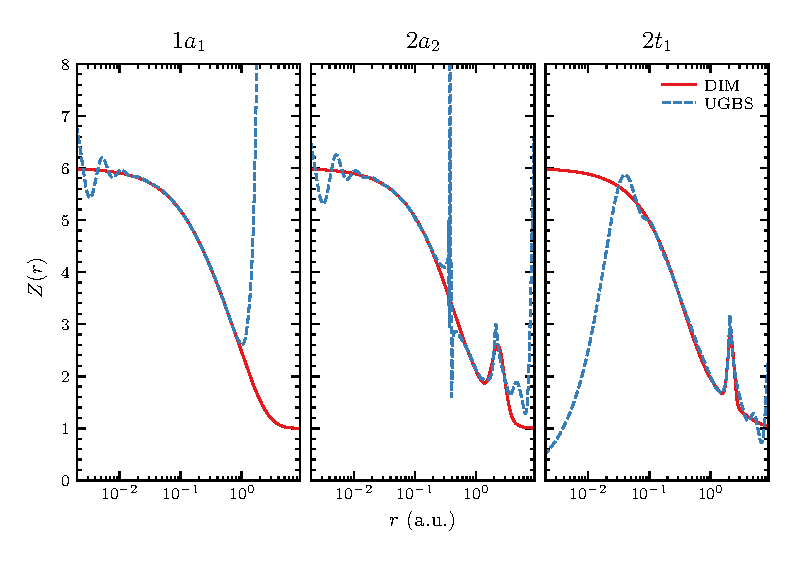
\includegraphics[width=0.9\textwidth]{figures/dim/ch4_dim.eps}
\caption[Cargas invertidas y depuradas de metano.]
{Cargas efectivas de CH$_4$ de los orbitales moleculares $1a_1$, $2a_2$ 
y $2t_1$ obtenidas a partir del conjunto de base UGBS; inversión directa 
(líneas discontinuas) e inversión depurada (líneas sólidas).}
\label{fig:ch4zeff}
\end{figure}

El ejemplo escogido para ilustrar la aplicación del DIM en moléculas es 
la molécula de metano. Este hidruro es lo suficientemente simétrico 
como para poder ser descripto por un potencial angular 
promediado~\cite{Granados:16}. 
Los orbitales moleculares HF de CH$_4$ se calculan usando los conjuntos 
de bases UGBS del carbono y el hidrógeno. Estas bases sólo consideran 
momentos angulares hasta $L=1$. El cálculo de estructura electrónica de 
metano con estos conjuntos de base deberían incluir funciones de 
polarización (por lo menos hasta las funciones $d$), con el fin de 
incrementar la precisión de las energías moleculares~\cite{Rothenberg:71,
Hariharan:72}. Sin embargo, para aislar los efectos de la base, éstos 
efectos no se incluyen aquí. 

Las cargas obtenidas mediante la inversión directa de los orbitales UGBS 
se muestran en la Fig.~\ref{fig:ch4zeff} con líneas discontinuas. Dado 
que los orbitales moleculares se describen a partir de combinaciones 
lineales de orbitales atómicos de hidrógeno y carbono, para remover los 
efectos de las bases, se deben determinar los perfiles de oscilación de 
de cada uno de los átomos constituyentes. Se emplea la 
Ec.~(\ref{eq:oscillation-prof}) para determinar los perfiles 
$p_{1s}^{\mbox{\scriptsize UGBS}}$, $p_{2s}^{\mbox{\scriptsize UGBS}}$ y 
$p_{2p}^{\mbox{\scriptsize UGBS}}$ del carbono. Así, se sustraen los 
perfiles $p_{nl}^{\mbox{\scriptsize UGBS}}$ de las correspondientes 
cargas invertidas $Z_{nl}^{\mbox{\scriptsize UGBS}}$ del metano. Las 
oscilaciones se remueven completamente para todos los orbitales excepto 
el $2a_2$, que presenta pequeñas fluctuaciones residuales debido a la 
base del hidrógeno. Ya que estas ondulaciones son mínimas y se ubican 
cerca del núcleo, éstas pueden ser despreciadas y se procede a 
implementar el método de depuración descripto en la 
Sección~\ref{sec:dimmoleculas}. 

Los parámetros de las cargas moleculares DIM definidos por la 
Ec.~(\ref{eq:molzDIM}) se presentan en la Tabla~\ref{tab:ch4parameters}. 
Las cargas correspondientes se muestran en la Fig.~\ref{fig:ch4zeff} con 
líneas sólidas. En este caso, la función de costo~(\ref{eq:fncosto-dim}) 
a minimizar considera los valores de energía y radios medios de los 
MOs dados por Moccia~\cite{Moccia:69} como valores conocidos. Las 
energías orbitales DIM reproducen estos valores hasta la cuarta cifra 
significativa y se dan en la Tabla~\ref{tab:ch4parameters}. Por otro 
lado, los radios medios $\langle r\rangle$ y $\langle 1/r\rangle$ 
obtenidos con los potenciales moleculares DIM están dentro del $1\%$ de 
los valores de Moccia.

\begin{table}[t]
\centering
\begin{tabular}{
>{\centering\arraybackslash}p{0.13\textwidth}
>{\centering\arraybackslash}p{0.13\textwidth}
>{\centering\arraybackslash}p{0.13\textwidth}
>{\centering\arraybackslash}p{0.13\textwidth}
>{\centering\arraybackslash}p{0.13\textwidth}
>{\centering\arraybackslash}p{0.13\textwidth}}
\rowcolor{mydarkgray} 
   $nl$ & $E$        & $z_j$        & $\alpha_j$   & $\beta$&$\gamma$\\
$1a_1$  & $-11.1949$ & $1.925280$ & $0.641982$ & & \\
\rowcolor{mygray} 
        &            & $0.953120$ & $5.571510$ & & \\
        &            & $2.121600$ & $1.500440$ & & \\
\rowcolor{mygray} 
$2a_2$  & $-0.9204$  & $2.912200$ & $3.149990$ & & \\
        &            & $2.087800$ & $0.771371$ & & \\
\rowcolor{mygray} 
        &            & $1.23640$  &            & $2.329570$&$0.053420$\\
$2t_1$  & $-0.5042$  & $0.901953$ & $2.895140$ & & \\
\rowcolor{mygray} 
        &            & $1.112030$ & $0.388649$ & & \\
        &            & $2.986017$ & $2.931210$ & & \\
\rowcolor{mygray} 
        &            & $1.301820$ &            & $2.169850$&$0.012616$\\ 
\end{tabular}
\caption[Energías y parámetros de ajuste de cargas efectivas de metano.]
{Energías orbitales moleculares y parámetros de ajuste de cargas 
efectivas de metano.}
\label{tab:ch4parameters}
\end{table}

%%%%%%%%%%%%%%%%%%%%%%%%%%%%%%%%%%%%%%%%%%%%%%%%%%%%%%%%%%%%%%%%%%%%%%%%
\subsection{Procesos colisionales simples}
%%%%%%%%%%%%%%%%%%%%%%%%%%%%%%%%%%%%%%%%%%%%%%%%%%%%%%%%%%%%%%%%%%%%%%%%
\label{subsec:procol}

Como aplicación del método de inversión depurada, se presenta el uso 
efectivo de los potenciales DIM para describir blancos multielectrónicos 
en procesos colisionales simples. En particular, se examina la 
ionización de atómos multielectrónicos y moléculas con pocos átomos 
debido al impacto de protones y fotones. 
Para esto, suponemos que el Hamiltoniano del sistema describe la 
dinámica del proyectil, el blanco y el electrón activo, y que el primer 
orden perturbativo de los elementos de la matriz de transición 
proporcionan una correcta representación en el rango intermedio--alto
de energía del proyectil incidente. El marco teórico de la ionización
está dada por la primera aproximación de Born (FBA). Además, en este 
orden de aproximación  y en el límite de altas energías, los orbitales 
de Hartree--Fock proporcionan una buena descripción de las secciones 
eficaces del blanco.
%En esta Sección se analiza la implementación del método de inversión 
%depurada para describir blancos atómicos y moleculares en procesos 
%colisionales simples. Los procesos colisionales se describen a primer 
%orden empleando la primera aproximación de Born (FBA). El rango de 
%validez de este método comprende las altas energías del proyectil 
%incidente. 
Por simplicidad, denominamos la combinación de la descripción del blanco 
mediante el potencial efectivo DIM y el modelado de la ionización a 
primer orden como ionización DIM-FBA. 

%=======================================================================
\subsubsection{Fotoionización}
%=======================================================================

Para demostrar la aplicabilidad del método DIM en procesos colisionales 
simples, se calcula la fotoionización de múltiples blancos atómicos y 
moleculares descriptos mediante potenciales DIM. De los sistemas 
estudiados, se escoge ilustrar los resultados para helio, nitrógeno, 
neón y metano. En la Fig.~\ref{fig:photoDIM} se muestran las secciones
eficaces de fotoionización DIM-FBA de los blancos seleccionados con 
líneas sólidas. Los resultados teóricos para helio y nitrógeno coinciden 
de manera excelente con los valores experimentales 
(símbolos)~\cite{Samson:90,Henke:93,Stolte:16} a bajas, medias y altas 
energías del fotón incidente. En el caso del átomo de neón, algunas 
discrepancias con las mediciones (símbolos) \cite{Henke:93,Samson:02} 
empiezan a surgir a energías bajas e intermedias del proyectil. Este 
comportamiento sugiere la necesidad de incluir en los cálculos de la 
fotoionización correcciones de mayor orden que incluyan efectos de 
múltiples cuerpos relevantes, tales como la relajación de los orbitales 
debido a la creación de un hueco electrónico, respuestas colectivas de 
electrones de capas internas~\cite{Ederer:64} y efectos de correlación.

\begin{figure}
\centering
\includegraphics[width=0.92\textwidth]{dim/fotoDIM-part1.eps} 

\vspace{-1.15cm}
\includegraphics[width=0.92\textwidth]{dim/fotoDIM-part2.eps}
\caption[Fotoionización de He, N, Ne y CH$_4$.]
{Sección eficaz total de fotoionización de un electrón de He, N, Ne y 
CH$_4$. Curvas: cálculos teóricos DIM-FBA. Símbolos: 
datos experimentales~\cite{Samson:90,Henke:93,Stolte:16,Samson:02,
Lukirskii:64,Henke:82,Samson:89}.}
\label{fig:photoDIM}
\end{figure}

En los blancos moleculares, la orientación molecular es importante para 
determinar la sección eficaz en un proceso colisional. Sin embargo, en 
la configuración experimental, las moléculas en estado gaseoso 
generalmente tienen orientaciones aleatorias. Por lo tanto, la 
descripción promediada esféricamente de los sistemas moleculares asumida 
por el potencial DIM está en concordancia con la configuración del 
blanco. En la región de energías entre $\sim$15 y 300 eV se aprecia la 
contribuación de la capa de valencia a la fotoionización, mientras que 
la discontinuidad en $0.3$~keV corresponde al umbral del orbital 
molecular $1a_1$. La predicción del modelo DIM-FBA para la sección 
eficaz total de fotonización de CH$_4$ se encuentra en buen acuerdo con 
valores experimentales~\cite{Lukirskii:64,Henke:82,Samson:89} en el 
rango de altas energías y cerca del umbral de la capa $2p$. Para 
fotoenergías bajas e intermedias, el acuerdo entre las predicciones 
DIM-FBA y los datos experimentales no es bueno. 
Los efectos colectivos mencionados anteriormente no han sido 
considerados en estos cálculos, y probablemente sean los responsables de 
las discrepancias observadas. En la fotoionización de un electrón 
perteneciente al orbital interno $1a_1$, estos efectos no son tan 
signficativos. De manera que, con sólo un primer orden de aproximación, 
se obtiene buen acuerdo con los valores experimentales disponibles. 

%=======================================================================
\subsubsection{Ionización por impacto de protones}
%=======================================================================

\begin{figure}[t]
\centering
\includegraphics[width=0.9\textwidth]{figures/dim/ionDIM.eps}
\caption[Ionización por impacto de protón de N y CH$_4$.]
{Sección eficaz total de ionización de un electrón por impacto de protón 
de N y CH$_4$. Línea sólida: cálculos teóricos DIM-FBA. 
Símbolos: datos experimentales de ionización por impacto de 
protón~\cite{Rudd:83,Rudd:85} y electrón~\cite{Brook:78} con conversión 
de equivelocidad.}
\label{fig:iondim}
\end{figure}

El uso efectivo de los potenciales DIM también se estudia examinando 
la ionización por impacto de protones en blancos multielectrónicos. De 
los cálculos realizados, se eligen dos ejemplos para ilustrar este 
proceso. Los resultados de ionización por impacto de protones para N y 
CH$_4$, en el marco del modelo DIM-FBA, se muestran en la 
Fig.~\ref{fig:iondim}. El acuerdo entre las predicciones teóricas y los 
datos experimentales~\cite{Rudd:83,Rudd:85} es muy bueno en la región de 
altas energías, donde tiene validez la primera aproximación de Born. En 
el caso de nitrógeno, se incluyen también datos experimentales de 
ionización por impacto de electrones~\cite{Brook:78}. Los valores de 
energía incidente de los electrones se convierten a partir del principio 
de equivelocidad, donde $m_p\approx 1836\,m_e$. Así, por ejemplo, 
electrones que inciden sobre el blanco con $0.54$~keV son equivalentes 
en energía a protones incidentes con aproximadamente 1~MeV. Para valores 
de energía mayores a 400~keV, la sección eficaz de ambos proyectiles 
coincide. 

%%%%%%%%%%%%%%%%%%%%%%%%%%%%%%%%%%%%%%%%%%%%%%%%%%%%%%%%%%%%%%%%%%%%%%%%
\section{Discusión: HF vs. DIM}
%%%%%%%%%%%%%%%%%%%%%%%%%%%%%%%%%%%%%%%%%%%%%%%%%%%%%%%%%%%%%%%%%%%%%%%%
\label{sec:discusionHF}

Las publicaciones de los resultados de este trabajo~\cite{Mendez:16,
Mendez:19dim,Mendez:18,Mitnik:19} han derivado en interesantes 
discusiones sobre la validez de las hipótesis del DIM respecto al 
comportamiento asintótico de las funciones de onda, y la posible 
existencia de potenciales locales. En esta Sección se repasan estas 
discusiones, examinando la teoría de Hartree--Fock y el origen de los 
defectos numéricos que surgen en los potenciales invertidos. Las 
hipótesis sobre las que se basa el método de inversión depurada permiten 
resolver estos defectos, por lo que se podría considerar al DIM como una 
alternativa para representar en forma precisa blancos atómicos a partir 
de potenciales locales.

Uno de los aspectos principales de esta discusión concierne la posible 
existencia (o la negación teórica) de un potencial local que pueda 
derivar a las funciones de onda originales de HF. Por ejemplo, el 
trabajo de Amusia \textit{et al.}~\cite{Amusia:04} concluye que esto es 
imposible ya que la densidad electrónica de Hartree--Fock no es 
$v$-representable y, por lo tanto, no se puede obtener como la densidad 
del estado fundamental de electrones no-interactuantes en un potencial 
local. Sin embargo, en este trabajo se ha demostrado que el método de 
inversión depurada permite obtener potenciales efectivos que reproducen 
con gran precisión las soluciones HF.

%%%%%%%%%%%%%%%%%%%%%%%%%%%%%%%%%%%%%%%%%%%%%%%%%%%%%%%%%%%%%%%%%%%%%%%%
\subsection{Nodos genuinos}
%%%%%%%%%%%%%%%%%%%%%%%%%%%%%%%%%%%%%%%%%%%%%%%%%%%%%%%%%%%%%%%%%%%%%%%%
\label{subsec:nodosHF}

Dado que el DIM se basa en la Ec.~(\ref{eq:Vinv}), en la cual la función de 
onda se encuentra en el denominador, el potencial invertido debería 
diverger en cada uno de los nodos del orbital excepto que se cumpla una 
condición específica: que derivadas segundas se anulen exactamente en 
esos mismos puntos. Esta condición no se asume en ninguna instancia de la 
teoría de Hartree--Fock. Sin embargo, durante esta investigación se han 
encontrado resultados que apuntan en esta dirección. Por ejemplo, en 
la Fig.~\ref{fig:example2sMg} se muestra la función 
$u_{2s}^{\mathrm{HF}}$ del Mg y su derivada segunda numérica (escalada 
por un factor). Las dos raíces de $u_{2s}^{\mathrm{HF}}''$ son puntos de 
inflexión de $u_{2s}^{\mathrm{HF}}$ y se corresponden a (1)~el nodo 
radial y (2)~el punto de retorno clásico en la función orbital. A 
primera vista, el nodo del orbital y la primera raíz de la derivada 
segunda parecen coincidir. Una inspección más cercana (ver recuadro) 
muestra que ese no es el caso. Definiendo $\Delta r$ como la distancia 
entre el nodo del orbital y la primera raiz de su derivada segunda, se 
encuentra una pequeña distancia $\Delta r=1\times 10^{-3}$~a.u. entre 
las primeras raíces de ambas funciones. Inspeccionando una gran cantidad 
de átomos, se encuentra que la proximidad entre estos dos puntos es 
general. Así, este comportamiento hace suponer que la cercanía entre los 
nodos genuinos de los orbitales HF y las correspondientes raíces de su 
segunda derivada no es casual, y que los nodos genuinos en la teoría de 
Hartree--Fock podrían también ser puntos de inflexión. 

\begin{figure}
\centering
\vspace{-0.45cm}
\includegraphics[width=0.85\textwidth]{dim/example_2sMg.eps} 
\vspace{-0.45cm}
\caption[Orbital radial y su derivada segunda.]
{Orbital radial $u_{2s}^{\mathrm{HF}}$ del estado fundamental de Mg y su 
derivada segunda escalada.}
\label{fig:example2sMg}
%\end{figure}
%\begin{figure}[t]
%\centering

\vspace{0.25cm}
\includegraphics[width=0.85\textwidth]{dim/dr_2sMg.eps} 
\vspace{-0.45cm}
\caption[Dependecia de $\Delta r$ del orden de aproximación numérica.]
{Dependecia de $\Delta r$ del orden de aproximación numérica en el 
orbital $2s$ del átomo de potasio. (a) Primer orden y 200 puntos, (b) 
400 puntos; (c) octavo orden y 1000 puntos.}
\label{fig:dr2sMg}
\end{figure}

Para indagar esta hipótesis, se diseña un experimento numérico que 
consiste en examinar el comportamiento del valor $\Delta r$ al realizar 
varias aproximaciones a los métodos usados para resolver las 
ecuaciones de HF. La calidad de estos métodos se evalúa variando el 
orden de precisión de los algoritmos y la densidad de puntos de las 
grillas numéricas. 
La Fig.~\ref{fig:dr2sMg} muestra $u_{2s}^{\mathrm{HF}}$ de Mg (línea 
sólida) y su segunda derivada numérica (línea discontinua) en las 
proximidades del nodo implementando tres grados de aproximación 
distintos en los métodos numéricos. Los cálculos menos precisos se 
muestran en la Fig.~\ref{fig:dr2sMg}(a), donde los algoritmos se 
implementan a primer orden y se usa una grilla numérica de 200 puntos 
(mínimo valor necesario para obtener convergencia), resultando en 
$\Delta r=8\times 10^{-3}$~a.u.. Aumentando el número de puntos a 400, 
este valor se reduce a $\Delta r=4\times 10^{-3}$~a.u., como se muestra 
en la Fig.~\ref{fig:dr2sMg}(b). Por último, se incrementa el número de 
puntos a 1000 y se usa el máximo orden de aproximación de los 
algoritmos. La Fig.~\ref{fig:dr2sMg}(c) muestra el mejor resultado 
posible, donde $\Delta r=1\times 10^{-3}$~a.u.. Aún considerando un 
número mayor de puntos en la grilla numérica, los resultados no varían. 
Se realizó un cálculo adicional usando el código \textsc{atomopm} de 
Talman, ampliamente implementado en la comunidad DFT. La 
Fig.~\ref{fig:dr2sMg}(c) muestra el orbital $u_{2s}^{\mathrm{OPM}}$ de 
Mg cerca del nodo con una línea raya-punto. Como se observa, su segunda 
derivada $u_{2s}^{\mathrm{OPM}}''$ (línea punto-raya-punto) es 
estrictamente cero en el nodo. Este resultado se debe a que el potencial
OPM es local. 

El presente experimento computacional sugiere que los nodos de los 
orbitales HF deberían ser puntos de inflexión. Para probar efectivamente 
esta hipótesis, será necesario considerar algoritmos con órdenes de 
aproximación mayores. De confirmarse, se podría modificar la teoría de 
Hartree--Fock agregando una restricción adicional al procedimiento 
variacional autoconsistente que asegure que los nodos sean además puntos 
de inflexión. En definitiva, el cumplimiento de esta restricción 
aseguraría la existencia de un potencial local, en principio, sin polos. 

%%%%%%%%%%%%%%%%%%%%%%%%%%%%%%%%%%%%%%%%%%%%%%%%%%%%%%%%%%%%%%%%%%%%%%%%
\subsection{Decaimiento exponencial}
%%%%%%%%%%%%%%%%%%%%%%%%%%%%%%%%%%%%%%%%%%%%%%%%%%%%%%%%%%%%%%%%%%%%%%%%
\label{subsec:decaimientoHF}

Otro aspecto teórico que ha derivado en interesantes discusiones dentro 
de la comunidad se refiere a las condiciones de borde~(\ref{eq:Zasympt}) 
que el método de inversión depurada impone a los potenciales invertidos. 
Esta discusión ha llegado a hacerse pública en un 
comentario~\cite{Cinal:19}, donde se objeta la validez del método de 
inversión depurada por este motivo.

En el DIM, el potencial se asume de tipo Coulombiano, con una carga 
efectiva en el origen determinada únicamente por la carga del núcleo. A 
grandes distancias, se supone que todos los electrones apantallan al 
núcleo dejando como resultado una carga efectiva igual a 1. De esta 
forma, a grandes distancias, los potenciales DIM están dados por
\begin{equation}
\lim_{r\rightarrow\infty} V_{nl}^{\mathrm{DIM}}(r) = -\frac{1}{r}\,.
\label{eq:VDIMasympt}
\end{equation}
Los orbitales correspondientes tienen un decaimiento asintótico 
denonimado en la literatura de ``tipo Hartree''~\cite{Casida:89},
\begin{equation}
\lim_{r \rightarrow \infty} u_{nl}^{\mathrm{DIM}}(r) \propto
\exp(- \sqrt{- 2 \varepsilon_{nl}^{\mathrm{HF}} } r ) \,.
\label{eq:uDIMasympt}
\end{equation}
El término ``tipo-Hartree'' puede resultar confuso ya que la energía 
del orbital $\varepsilon_{nl}^{\mathrm{HF}}$ se corresponde a valores 
donde se ha considerado el término de intercambio. 

Sin embargo, en la teoría de HF, los orbitales tienen un comportamiento 
asintótico diferente, dictado por la energía del orbital molecular de 
mayor ocupación (\acs{homo}) $\varepsilon_{\mathrm{HOMO}}^{\mathrm{HF}}$ 
\cite{Handy:69,Handler:80,Ishida:92},
\begin{equation}
\lim_{r \rightarrow \infty} u_{nl}^{\mathrm{HF}}(r) \propto
\exp(- \sqrt{- 2 \varepsilon_{\mathrm{HOMO}}^{\mathrm{HF}} } r )  \, .
\label{eq:uHFasympt}
\end{equation}
Este comportamiento se debe al potencial \textit{exacto} de 
Hartree--Fock~\cite{Cinal:10}, que está dado por
\begin{equation}
\lim_{r\rightarrow\infty} V_{nl}^{\mathrm{HF}}(r) \approx
-\left(\varepsilon_{\mathrm{HOMO}}^{\mathrm{HF}}
-\varepsilon_{nl}^{\mathrm{HF}}\right)+\frac{q_{nl}}{r}\,,
\label{eq:VHFasympt}
\end{equation}
donde $\varepsilon_{nl}$ son las energías orbitales de HF y $q_{nl}$ es 
un coeficiente que depende del orbital y puede ser distinto de $-1$.

El comportamiento asintótico de los orbitales~(\ref{eq:uHFasympt}) y el 
potencial exacto~(\ref{eq:VHFasympt}) de Hartree--Fock se han demostrado 
rigurosamente. Sin embargo, muchos autores han puesto en tela de juicio 
su relevancia, interpelando si este comportamiento \textit{tiene un 
significado físico o si es 
sólo un artefacto del método de Hartree--Fock}\myfnote{}~\cite{Handy:69}. 
Handler y Smith reconocieron estos cuestionamientos señalando que el 
\textit{la cuestión del comportamiento asintótico es de interés 
intrínseco de la teoría}\myfnote{}~\cite{Handler:80}.
Weber y Parr estudiaron en profundidad este problema: limitaron los 
efectos de intercambio entre electrones a una ``esfera de influencia''
finita y asumieron que \textit{el electrón que se extrae de un átomo es 
de alguna manera distinguible por el hecho de la separación. De cierta 
forma, este electrón ve al ion como una carga positiva clásica si la 
distancia entre ellos es lo suficientemente grande y, por lo tanto, en 
este contexto, los efectos de intercambio pueden 
despreciarse}\myfnote{}~\cite{Weber:71}.

\begin{figure}
\centering
\includegraphics[width=0.85\textwidth]{dim/V1s_K.eps} 
\caption[Comportamiento asintótico de los potenciales.]
{Comportamiento asintótico de los potenciales invertido HF (línea 
discontinua) y DIM (línea sólida) de orbital $1s$ del átomo de K.}
\label{fig:V1sK}
\end{figure}

A continuación, se presenta un ejemplo que permite ilustrar estos 
conceptos en forma concreta. En la Fig.~\ref{fig:V1sK} se muestran los 
potenciales $V_{1s}^{\mathrm{DIM}}$ y $V_{1s}^{\mathrm{HF}}$ del átomo 
de potasio con líneas sólida y discontinua, respectivamente. El punto de 
retorno clásico del orbital $1s$ se ilustra con una línea vertical 
punteada: a partir de allí, el orbital decae exponencialmente. En la 
región asintótica, el potencial invertido tiende a una constante, 
siguiendo la Ec.~(\ref{eq:VHFasympt}). Por ello, cuando los potenciales 
se reescriben en términos de cargas efectivas, estas últimas divergen 
(ver recuadro). Sin embargo, el potencial DIM tiene, por definición, una 
forma Coulombiana y la carga efectiva tiende a 1 a grandes distancias, 
siguiendo la Ec.~(\ref{eq:VDIMasympt}).

\begin{figure}[t]
\centering
\includegraphics[width=0.85\textwidth]{dim/Lns_K.eps} 
\caption[Comportamiento asintótico de los orbitales HF.]
{Comportamiento asintótico de los orbitales HF (líneas discontinuas y 
sólidas) y DIM (líneas punteadas) según $L_{nl}$, dada por la 
Ec.~(\ref{eq:Lnl}), de los orbitales $s$ del átomo de K.}
\label{fig:LnsK}
\end{figure}

En la región asintótica, la amplitud de los orbitales es miníscula y 
resulta conveniente examinar su comportamiento en detalle a través de la 
derivada logarítmica, 
\begin{equation}
L_{nl}(r) \equiv r \frac{d \log{u_{nl}}}{d r}\,,
\label{eq:Lnl}
\end{equation}
que debería tener una forma lineal para funciones $u_{nl}$ que decaen 
exponencialmente. Siguiendo el ejemplo anterior, la Fig.~\ref{fig:LnsK} 
ilustra la derivada logarítmica de los orbitales HF $ns$ del átomo de 
potasio. Los orbitales HF se muestran con líneas discontinuas (capas 
internas $1s$, $2s$ y $3s$) y sólidas (capa de valencia $4s$). 
Los polos de las funciones $L_{nl}(r)$ corrresponden a los nodos de las 
funciones $u_{nl}$. La relación del número cuántico radial establece que 
los orbitales $1s$ no tienen nodos, mientras que los orbitales $2s$ 
tienen sólo uno. Sin embargo, en el caso de potasio, el orbital $1s$ 
presenta dos polos, i.e. dos nodos espurios, en $0.99$~a.u. y 
$5.68$~a.u.. Además, el orbital $2s$ tiene un nodo espurio en 
$5.78$~a.u.. Estos nodos se discuten en la siguiente Sección.

A grandes distancias, $r>10$~a.u., los orbitales de K de la 
Fig.~\ref{fig:LnsK} presentan el comportamiento de HF dado por la 
Ec.~(\ref{eq:uHFasympt}): los orbitales de las capas internas y el 
\acs{homo} son indistinguibles. Además, se incluye la región asintótica 
de los orbitales DIM $1s$, $2s$ y $3s$ (líneas punteadas), que presentan 
el decaimiento exponencial de ``tipo Hartree'' dado por la 
Ec.~(\ref{eq:uDIMasympt}). Se observa que las funciones 
$u_{nl}^{\mathrm{HF}}$ tienen el mismo decaimiento exponencial que las 
funciones DIM a partir del punto de retorno clásico de cada orbital y 
hasta $0.4$~a.u., $1.5$~a.u. y 5~a.u. en los orbitales $1s$, $2s$ y 
$3s$, respectivamente. Por lo tanto, el comportamiento físico más 
importante de los orbitales en la región asintótica está dictada por la 
expresión de ``tipo Hartree'', en lugar del comportamiento exacto de la 
teoría de Hartree--Fock. Esta es quizás la razón por la que Weber, Handy 
y Parr~\cite{Weber:70} sugirieron considerar el comportamiento de largo 
alcance~(\ref{eq:uDIMasympt}) como deseable, produciendo resultados más 
precisos que los obtenidos por la teoría formal de HF. Al inspeccionar 
la espectroscopía electrónica experimental ($e$,$2e$), Casida y 
Chong~\cite{Casida:89} también llegaron a las mismas conclusiones. 

La discusión sobre qué condición asintótica es la más apropiada todavía 
no está saldada. Sin embargo, la definición de las condiciones de borde 
del DIM siguen a Weber, Handy y Parr, que sugieren que el comportamiento 
a grandes distancias~(\ref{eq:VDIMasympt}) es preferible y produce 
resultados más precisos que los que otorga la teoría formal de 
Hartree--Fock. 

%%%%%%%%%%%%%%%%%%%%%%%%%%%%%%%%%%%%%%%%%%%%%%%%%%%%%%%%%%%%%%%%%%%%%%%%
\subsection{Nodos espurios}
%%%%%%%%%%%%%%%%%%%%%%%%%%%%%%%%%%%%%%%%%%%%%%%%%%%%%%%%%%%%%%%%%%%%%%%%
\label{subsec:espuriosHF}

Las implicancias de asumir el potencial exacto de HF a grandes 
distancias tiene efectos inesperados en los orbitales radiales: surgen
oscilaciones espurias en la región asintótica. Hay escasas referencias 
en la teoría de Hartree--Fock sobre la existencia de los nodos espurios. 
Por ejemplo, Fischer~\cite{FroeseFischer:97} los menciona brevemente, 
aunque sin proporcionar detalles posteriores. 
%Nótese que los nodos espurios aparecen, en principio, como resultado 
%del cambio en el decaimiento asintótico de tipo 
%Hartree~(\ref{eq:uDIMasympt}) al de Hartree--Fock~(\ref{eq:uHFasympt}), 
%que incluye formalmente el intercambio.

La existencia de los nodos espurios en los orbitales HF no se debe al 
esquema numérico sino que es inherente al método. 
Lo hemos comprobado calculando orbitales con diferentes métodos e 
implementaciones. En todos los cálculos realizados con \textsc{hf} y 
\texthf{nrhf}, se encontraron los mismos nodos espurios exactamente en 
los mismos puntos. Incluso coinciden con los escasos reportes que se 
encuentran en la literatura, independientemente del método empleado para 
resolver las ecuaciones de HF.  Los cálculos que emplean bases 
introducen muchos mas nodos, pero dada la representación finita de las 
bases, estos cálculos no son confiables a grandes distancias.
En general, estos nodos aparecen en regiones donde los valores de
$r$ son grandes y las amplitudes de los orbitales son despreciables.
La teoría de Hartree--Fock se basa en el principio variacional, por lo 
que el comportamiento asintótico de los orbitales tiene un efecto 
insignificante en los valores medios de las soluciones, particularmente, 
en las energías. Por lo tanto, su existencia no tiene consecuencias 
prácticas y se pueden, y deben, ignorar en cualquier cálculo HF. 
Sin embargo, en el esquema de inversión, el ancho y la amplitud de los 
nodos espurios afectan significativamente las regiones más internas de 
la carga invertida. Por ejemplo, el nodo espurio del orbital $2s$ del 
átomo de potasio ubicado en $r\approx 5.78$~a.u., que se muestra en el 
recuadro de la Fig.~\ref{fig:2sK}(a), es traducido por la inversión como
un polo. Más aún, la presencia del nodo espurio afecta la carga de 
manera tal que ésta empieza a diverger a partir $r\approx 1$~a.u., donde 
la amplitud del orbital no es lo suficientemente pequeña. 

Quizás el cuestionamiento más importante al DIM gira alrededor del hecho 
que el método adopta el comportamiento de ``tipo Hartree'' en lugar del 
comportamiento asintótico que dicta la teoría de Hartree--Fock. El 
trabajo de Weber \textit{et al.}~\cite{Weber:70} plantea una importante 
conjetura al respecto. Los autores teorizaron que todos los signos de 
los nodos espurios desaparecerían cuando los orbitales tuvieran un 
comportamiento asintótico de ``tipo Hartree'', en lugar del límite 
exacto~(\ref{eq:uHFasympt}). La condición de borde asintótica del DIM 
va en consonancia con esta hipótesis y los orbitales DIM no presentan 
nodos espurios.

\begin{center}
\rule[0.5ex]{0.8\linewidth}{0.5pt}
\end{center}

Las discusiones de esta Sección se pueden resumir en las siguientes 
afirmaciones:
\begin{itemize}
\item La existencia de un potencial local de Hartree--Fock es 
cuestionable ya que la densidad de HF no es $v$-representable.
\item La hipótesis de que los nodos de los orbitales y las raices 
correspondientes de su derivada segunda deben coincidir aseguraría, en 
principio, la existencia de un potencial local sin nodos.
%\item Los potenciales exactos de HF no se pueden expresar con una forma 
%Coulombiana ya que lejos del núcleo tienden a una constante.
\item El correcto límite asintótico que deben seguir las funciones 
radiales orbitales es todavía sujeto de discusión. 
\item La existencia de los nodos espurios se debe al término de 
intercambio que sobrevive a grandes distancias, y dicta el 
comportamiento del potencial exacto en la teoría de HF.
\item A diferencia del método HF, el límite asintótico del potencial DIM 
permite representar el apantallamiento electrónico de forma correcta.
\item Los orbitales DIM siguen las condiciones asintóticas de ``tipo 
Hartree'' y no presentan nodos espurios, los cuales son intrínsecos a la 
teoría de HF.
\end{itemize}
Así, el comportamiento ``tipo Hartree'' asumido para los potenciales DIM 
se considera el más apropiado ya que permiten describir correctamente 
los orbitales y sus condiciones de borde. Además, el método asegura 
potenciales locales, que reproducen las soluciones HF en forma precisa
y se pueden usar para describir procesos colisionales simples, lo que 
constituye el objetivo principal de este trabajo.

\begin{comment}

%%%%%%%%%%%%%%%%%%%%%%%%%%%%%%%%%%%%%%%%%%%%%%%%%%%%%%%%%%%%%%%%%%%%%%%%
\subsection{Conclusiones}
%%%%%%%%%%%%%%%%%%%%%%%%%%%%%%%%%%%%%%%%%%%%%%%%%%%%%%%%%%%%%%%%%%%%%%%%

En esta Sección se presentaron los detalles teóricos del origen de los
defectos que presentan los potenciales invertidos HF. Se encontró que 
estos defectos surgen del propio método de Hartree--Fock: 
\begin{itemize}
\item Los nodos genuinos de los orbitales HF no son estrictamente puntos 
de inflexión.
\item Si bien el decaimiento exponencial de los orbitales sigue 
inicialmente el comportamiento orbitales tipo Hartree, éstos luego son 
forzados por la teoría a un comportamiento que no da cuenta del 
apantallamiento electrónico.
\item El cambio en el decaimiento exponencial conduce a la aparición de 
nodos espurios.
\end{itemize}
El análisis presentado aquí conduce a concluir que los potenciales que 
se obtienen de la inversión de orbitales Hartree--Fock no existen. El 
operador de Fock, que le imprime al método la no localidad, elimina toda 
posibilidad de la existencia de un potencial HF local. En 
contraposición, los potenciales DIM reproducen las soluciones de HF con 
gran precisión a la vez que cumplen con la correcta descripción del 
blanco: los nodos de los orbitales son puntos de inflexión, éstos no 
tienen nodos espurios y, lejos del núcleo, el apantallamiento del 
electrón es igual a uno. Así, teniendo en mente que el objetivo de 
nuestro trabajo constituye encontrar potenciales que permitan 
representar los estados inicialmente y finales del blanco en un proceso 
colisional de forma directa, se puede inferir que el método de inversión 
depurada constituye de alguna manera una instancia superior al método de 
Hartree--Fock, ya que permite definir potenciales locales con soluciones 
precisas.




\newpage
\subsection*{Inversión de orbitales HF a grandes distancias}

Por simplicidad, suponiendo que tengo el orbital HF $ns$, la ecuación de 
inversión~(\ref{eq:Vinv}) resulta
\begin{equation}
V_{ns}(r) = \frac{1}{2\,u_{ns}}\frac{d^2\,u_{ns}}{dr^2}
+\varepsilon_{ns}\,.
\end{equation}
El comportamiento asintótico de estos orbitales HF está dado por
\begin{equation}
\lim_{r\rightarrow\infty} u_{ns}(r) = e^{-\alpha r}\,,
\end{equation}
donde $\alpha=\sqrt{-2\varepsilon_{\mathrm{HOMO}}}$. Entonces, el 
potencial invertido resulta
\begin{align}
\lim_{r\rightarrow\infty}V_{ns}(r) 
&=\frac{1}{2}\frac{1}{e^{-\alpha r}}\frac{d^2\,
\left(e^{-\alpha r}\right)}{dr^2}+\varepsilon_{ns} \\
&=\frac{\alpha^2\,\cancel{e^{-\alpha r}}}{2\cancel{e^{-\alpha r}}}
+\varepsilon_{ns} \\
&=\frac{-2\varepsilon_{\mathrm{HOMO}}}{2}+\varepsilon_{ns} \\
&=-\left(\varepsilon_{\mathrm{HOMO}}-\varepsilon_{ns}\right) \\
&=-C < 0 \quad\forall(ns\neq \mathrm{HOMO})\,.
\end{align}
Entonces, en el límite de grandes distancias, el potencial invertido no 
es cero sino constante. Cuando supongo que tiene forma Coulombiana,
\begin{equation}
\lim_{r\rightarrow\infty} Z_{ns}(r) = C\,r\,\Rightarrow\,
\mbox{divergencia lineal (C es positivo)} \,.
\end{equation}
\end{comment}




